% \documentclass{beamer}
%Для защит онлайн лучше использовать разрешение 16x9
\documentclass[aspectratio=169]{beamer}

%%% PDF settings
\pdfvariable minorversion 7 % Set PDF version to 1.7.

%%% Fonts and language setup.
\usepackage{polyglossia}
% Setup fonts.
\usepackage{fontspec}
\setmainfont{CMU Serif}
\setsansfont{CMU Sans Serif}
\setmonofont{CMU Typewriter Text}

\usepackage{microtype} % Add fancy-schmancy font tricks

\usepackage{xcolor} % Add colors support.

%% Math
\usepackage{amsmath, amsfonts, amssymb, amsthm, mathtools} % Advanced math tools.
\usepackage{thmtools}
\usepackage{unicode-math} % Allow TTF and OTF fonts in math and allow direct typing unicode math characters.
\unimathsetup{
    warnings-off={
            mathtools-colon,
            mathtools-overbracket
        }
}
\setmathfont{Latin Modern Math} % default
\setmathfont[range={\setminus,\varnothing,\smashtimes}]{Asana Math}

%%% Images
\usepackage{graphicx}
\graphicspath{{figures/}}
\usepackage{import}

%%% Polyglossia setup after (nearly) everything as described in documentation.
\setdefaultlanguage{russian}
\setotherlanguage{english}

\usepackage{csquotes}

%%% Custom commands
\newcommand{\R}{\mathbb{R}}
\newcommand{\N}{\mathbb{N}}
\newcommand{\Z}{\mathbb{Z}}
\newcommand{\Q}{\mathbb{Q}}
\newcommand{\C}{\mathbb{C}}
\newcommand{\id}{\mathrm{id}}
\AtBeginDocument{\renewcommand{\leq}{\leqslant}}
\AtBeginDocument{\renewcommand{\geq}{\geqslant}}
\AtBeginDocument{\renewcommand{\Re}{\operatorname{Re}}}
\AtBeginDocument{\renewcommand{\Im}{\operatorname{Im}}}
\AtBeginDocument{\renewcommand{\phi}{\varphi}}
\AtBeginDocument{\renewcommand{\epsilon}{\varepsilon}}

%%% theorem-like envs
\theoremstyle{definition}

\declaretheoremstyle[spaceabove=0.5\topsep,
    spacebelow=0.5\topsep,
    headfont=\bfseries\sffamily,
    bodyfont=\normalfont,
    headpunct=.,
    postheadspace=5pt plus 1pt minus 1pt]{myStyle}
\declaretheoremstyle[spacebelow=\topsep,
    headfont=\bfseries\sffamily,
    bodyfont=\normalfont,
    headpunct=.,
    postheadspace=5pt plus 1pt minus 1pt,]{myStyleWithFrame}
\declaretheoremstyle[spacebelow=\topsep,
    headfont=\bfseries\sffamily,
    bodyfont=\normalfont,
    headpunct=.,
    postheadspace=5pt plus 1pt minus 1pt,
    qed=\blacksquare]{myProofStyleWithFrame}

\usepackage[breakable]{tcolorbox}
\tcbset{sharp corners=all, colback=white}
% \tcolorboxenvironment{theorem}{}
% \tcolorboxenvironment{theorem*}{}
% \tcolorboxenvironment{axiom}{}
% \tcolorboxenvironment{assertion}{}
% \tcolorboxenvironment{lemma}{}
% \tcolorboxenvironment{proposition}{}
% \tcolorboxenvironment{corollary}{}
% \tcolorboxenvironment{definition}{}
% \tcolorboxenvironment{proofReplace}{toprule=0mm,bottomrule=0mm,rightrule=0mm, colback=white, breakable }

\declaretheorem[name=Теорема, style=myStyleWithFrame]{theorem}
\declaretheorem[name=Теорема, numbered=no, style=myStyleWithFrame]{theorem*}
\declaretheorem[name=Аксиома, sibling=theorem, style=myStyleWithFrame]{axiom}
\declaretheorem[name=Преположение, sibling=theorem, style=myStyleWithFrame]{assertion}
\declaretheorem[name=Лемма, style=myStyleWithFrame]{lemma}
\declaretheorem[name=Предложение, sibling=theorem, style=myStyleWithFrame]{proposition}
\declaretheorem[name=Следствие, numberwithin=theorem, style=myStyleWithFrame]{corollary}

\declaretheorem[name=Определение, style=myStyleWithFrame]{definition}
\declaretheorem[name=Свойство, style=myStyle]{property}
\declaretheorem[name=Свойства, numbered=no, style=myStyle]{propertylist}

\declaretheorem[name=Пример, style=myStyle]{example}
\declaretheorem[name=Замечание, numbered=no, style=myStyle]{remark}

\declaretheorem[name=Доказательство, numbered=no, style=myProofStyleWithFrame]{proofReplace}
\renewenvironment{proof}[1][\proofname]{\begin{proofReplace}}{\end{proofReplace}}
% \declaretheorem[name=Доказательство, numbered=no, style=myProofStyleWithFrame]{longProof}

%%% Memoir settings
\chapterstyle{ger}
\setlength{\headheight}{2\baselineskip}

%%% HyperRef
\usepackage{hyperref}


\usepackage{tabularx}
\usepackage{booktabs}

% То, что в квадратных скобках, отображается внизу по центру каждого слайда.
\title[Lamagraph]{Разработка инфраструктуры для создания специализированных ускорителей на основе Interaction Nets}

% То, что в квадратных скобках, отображается в левом нижнем углу.
\institute[СПбГУ]{}

% То, что в квадратных скобках, отображается в левом нижнем углу.
\author{Ефим Кубышкин \and Николай Пономарев}

\date{}

\begin{document}
{
\setbeamertemplate{footline}{}
% Лого университета или организации, отображается в шапке титульного листа
\begin{frame}
    
\includegraphics[width=1.4cm]{pictures/SPbGU_Logo.png}
    \vspace{-35pt}
    \hspace{-10pt}
    \begin{center}
        \begin{tabular}{c}
            \scriptsize{Санкт-Петербургский государственный университет} \\
            \scriptsize{Кафедра системного программирования}
        \end{tabular}
        \titlepage
    \end{center}

    \btVFill

    \begin{center}
        \vspace{5pt}
        \scriptsize{Санкт-Петербург\\
            2025}
    \end{center}

\end{frame}
}

\begin{frame}{Введение}
    \begin{itemize}
        \item Современные вычислительные системы сталкиваются с растущей потребностью в параллельной обработке данных
        \item Традиционные архитектуры процессоров неэффективны для нерегулярного параллелизма
        \item[\faThumbsUp] Interaction Nets — формализм, предложенный Ивом Лафоном в 1989 году, для которого нерегулярный параллелизм естественен
        \item[\faThumbsDown] На данный момент существуют только программные реализации
    \end{itemize}
\end{frame}

\begin{frame}{Interaction Nets}

    \begin{columns}
        \begin{column}{0.65\linewidth}
            \begin{itemize}
                \item Математическая модель, основанная на графовых грамматиках
                \item Переписывания (редукции) независимы
                \item Доказана полнота по Тьюрингу и свойство независимости от порядка вычислений
                \item Метки на вершинах и правила грамматики можно менять $\Rightarrow$ высокая степень параметризуемости
            \end{itemize}
        \end{column}
        \begin{column}{0.3\linewidth}
            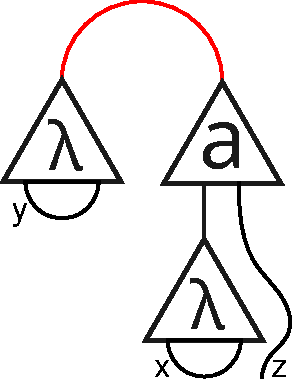
\includegraphics[width=\linewidth]{pictures/lamda-graph.pdf}
        \end{column}
    \end{columns}
\end{frame}

\begin{frame}
    \frametitle{Цель и задачи проекта}
    % \begin{enumerate}
    %     \item Сколько ресурсов ПЛИС будет занимать Interaction Nets?
    %     \item
    % \end{enumerate}

    \textbf{Цель:} Разработка параметризуемого многоядерного вычислителя на основе Interaction Nets

    \vspace{2em}

    Этапы достижения цели:
    \begin{description}
        \item[\only<2->{\faArrowRight{}} 1.] Создание минимальной инфраструктуры для создания специализированных вычислителей на основе Interaction Nets
              \only<2->{
                  \begin{itemize}
                      \item Реализация высокоуровневого языка программирования
                      \item Разработка транслятора из высокоуровневого языка в Interaction Nets
                      \item Реализация интерпретатора Interaction Nets
                      \item Разработка генератора прошивки вычислителя для ПЛИС
                  \end{itemize}
              }
        \item[2.]<1> Разработка eDSL для спецификации Interaction Nets
        \item[3.]<1> Добавление поддержки многоядерности
        \item[4.]<1> Проведение экспериментов
    \end{description}

    % \textbf{Гипотеза:} реализация в железе системы, поддерживающей нерегулярный параллелизм, позволит оптимизировать (по времени) исполнение задач искусственного интеллекта, анализа графов и разреженной линейное алгебры

    % \vspace{2em}
    % \textbf{Исследовательские вопросы:}
    % \begin{description}
    %     \item[RQ1] ... (это очень странно, но мы нихрена не можем сформулировать ркушки)
    % \end{description}
\end{frame}

\begin{frame}
    \frametitle{Требования к первому этапу}

    \begin{itemize}
        \item Использование единого стека технологий~--- гомогенность
              \begin{itemize}
                  \item Упрощение цепочки обработки данных
              \end{itemize}
        \item Получение полнофункционального прототипа, содержащего все компоненты, важнее, чем детальная проработка какого-то отдельного компонента
              \begin{itemize}
                  \item Фокус на инфраструктуре
                  \item Сбор информации о трудностях на каждом этапе
              \end{itemize}
        \item Возможность сбора статистики
              \begin{itemize}
                  \item Исследовательский проект
              \end{itemize}
              % \item На каждом этапе можем получить какой-то результат, значит можем тестировать
        \item Итеративность: на каждом этапе есть результат исполнения программы
              \begin{itemize}
                  \item Тестирование каждой из компонент
                  \item Сравнение результатов работы компонент
              \end{itemize}
    \end{itemize}

\end{frame}

\begin{frame}
    \frametitle{Lamagraph}

    \begin{figure}
        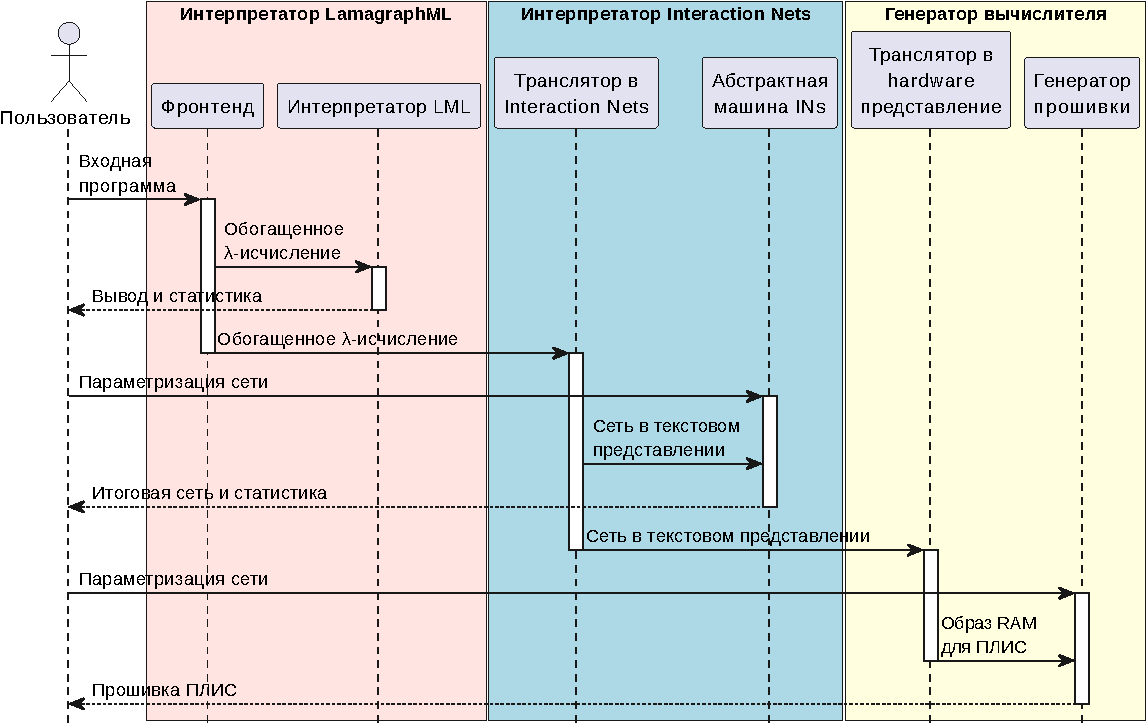
\includegraphics[width=0.75\linewidth]{pictures/using.pdf}
    \end{figure}

\end{frame}

\begin{frame}
    \frametitle{Интерпретатор LamagraphML}

    \begin{itemize}
        \item Проекты, реализующие Interaction Nets, обычно ставят своей целью реализацию интерпретатора Interaction Nets
        \item Поэтому для программирования используют собственные языки программирования, часто довольно сложные и синтаксически далёкие от массовых
        \item Мы же хотим использовать Interaction Nets как ассемблер, выдав программисту высокоуровневый язык
        \item Выбор именно функциональной парадигмы продиктован "близостью" Interaction Net к $\lambda$-исчислению, и бОльшими возможностями к параллелизму (чистота функций)
        \item Синтаксис высокоуровневого языка основан на ML с системой типов Хиндли-Милнера
        \item Фронтенд выдаёт обогащенное $\lambda$-исчисление, которое а) интерпретируется; б) перегоняется в Interaction Nets
    \end{itemize}

\end{frame}

\begin{frame}
    \frametitle{Интерпретаторы Interaction Nets}

    \begin{itemize}
        \item Используется текстовое представление Interaction Nets
        \item State-of-the-art наука умеет транслировать только чистое $\lambda$-исчисление
    \end{itemize}

    \vspace{1em}

    \begin{columns}[t]
        \begin{column}{0.5\linewidth}
            Исходных терм: \[(\lambda x. x) (\lambda y. y)\]

            Текстовое представление:
            \[\big\langle z \mid a(z, \lambda(x, x)) = \lambda(y, y) \big\rangle\]
        \end{column}
        \begin{column}{0.5\linewidth}
            Графическое представление:
            \begin{figure}
                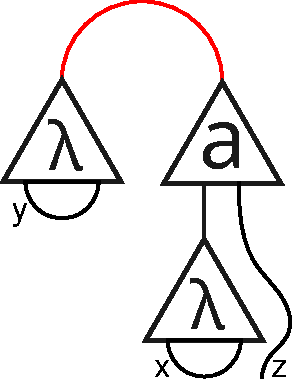
\includegraphics[width=0.4\linewidth]{pictures/lamda-graph.pdf}
            \end{figure}
        \end{column}
    \end{columns}

\end{frame}

\begin{frame}
    \frametitle{Генератор вычислителя}
    % \framesubtitle{Clash}

    \begin{itemize}
        \item Clash~--- язык описания программного обеспечения, основанный на Haskell
              \begin{itemize}
                  \item Unit тесты для комбинационной логики
                  \item Симуляция последовательностной логики
                  \item Test bench файлы на Verilog
              \end{itemize}
        \item Сбор статистики
              \begin{itemize}
                  \item Количество тактов
                  \item Количество редукций
                  \item Максимальный размер сети
              \end{itemize}
        \item Параметризация правилами переписывания и метками на узлах через типы
    \end{itemize}
\end{frame}

\begin{frame}
    \frametitle{Текущий статус}

    \begin{itemize}
        \item[] \textbf{Программа на LamagraphML}
              \begin{itemize}
                  \item[\faCheck] Интерпретация
                  \item[\faCogs] Трансляция в Interaction Nets (только $\lambda$-исчисление)
              \end{itemize}
        \item[] \textbf{Абстрактная машина}
              \begin{itemize}
                  \item[\faCheck] Интерпретация
                  \item[\faCheck] Сбор статистики
                        %   \item[\faCheck] Параметризация сетей
              \end{itemize}
        \item[] \textbf{Генерация вычислителя}
              \begin{itemize}
                  \item[\faCheck] Прошивка вычислителя для ПЛИС
                  \item[\faCheck] Сбор статистики
                        %   \item[\faCheck] Параметризация сетей
                        %   \item[\faCheck] Тесты, симуляция
              \end{itemize}
    \end{itemize}
    % \begin{table}
    %     \begin{tabularx}{\linewidth}{l>{\raggedright\arraybackslash}X}
    %         \toprule
    %         Этап                      & Возможности                                                                                                                                         \\
    %         \midrule
    %         Высокоуровневая программа & Тестирование, интерпретация, трансляция в Interaction Nets (только $\lambda$-исчисление)                                                            \\
    %         % Транслятор в Interaction Nets & только чистое $\lambda$-исчисление  \\
    %         Абстрактная машина        & Интерпретация (только $\lambda$-исчисление), сбор статистики, параметризация сетей                                                                  \\
    %         Вычислитель               & Интерпретация (только $\lambda$-исчисление), сбор статистики, параметризация сетей, тестирование в симуляторе, тестирование в test bench на Verilog \\
    %         \bottomrule
    %     \end{tabularx}
    % \end{table}

\end{frame}

% \begin{frame}{Clash}

%   % \vspace{5mm}
%   \begin{itemize}
%     \item Язык описания программного обеспечения, основанный на Haskell
%     \item Активно использует программирование на типах
%     \item Транслируется в SystemVerilog, Verilog или VHDL
%     \item Позволяет симулировать код и тестировать без написания test bench
%   \end{itemize}
% \end{frame}

% % \begin{frame}{Обзор}
% %   \begin{itemize}
% %     \item \textbf{Interaction Nets}:
% %           \begin{itemize}
% %             \item Математическая модель, поддерживающая параллельные вычисления.
% %             \item Вычисления происходят через редукции (переписывание графов).
% %             \item Пример: реализация $\lambda$-исчисления через Interaction Nets.
% %           \end{itemize}
% %     \item \textbf{Программные реализации}:
% %           \begin{itemize}
% %             \item INPLA, HVM — программные реализации Interaction Nets.
% %             \item Ограничены традиционными архитектурами.
% %           \end{itemize}
% %     \item \textbf{CLASH}:
% %           \begin{itemize}
% %             \item Язык для описания цифровых схем на основе Haskell.
% %             \item Упрощает разработку и тестирование аппаратных решений.
% %           \end{itemize}
% %   \end{itemize}
% % \end{frame}

% % Словами то, что в тексте
% \begin{frame}{Общая архитектура}
%   \begin{itemize}
%     \item Над проектом работает два человека
%     \item Данная работа фокусируется на Hardware компоненте
%   \end{itemize}
%   \begin{figure}
%     \includegraphics[width=\linewidth]{pictures/lamagraph-big-horiz.pdf}
%     \label{big_mmd}
%     % \caption{Общая схема зависимостей проекта}
%   \end{figure}
% \end{frame}

% \begin{frame}{Требования к проекту}
%   \begin{itemize}
%     \item  Параметризация всех компонентов типами агентов сети и правилами их редукции
%     \item Возможность сбора статистики
%     \item Возможность постановки сравнительных экспериментов
%     \item Использование единого стека технологий — гомогенность
%     \item Получение полнофункционального прототипа, содержащего все компоненты,
%           важнее, чем детальная проработка какого-то отдельного компонента
%     \item Расширяемость и модифицируемость
%   \end{itemize}
% \end{frame}

% \begin{frame}{Постановка задачи}

%   \textbf{Цель:}  Реализация параметризуемого вычислителя на основе Interaction Nets

%   \vspace{5mm}
%   \textbf{Задачи:}
%   \begin{enumerate}
%     \item Спроектировать инфраструктуру
%     \item Спроектировать общую архитектуру проекта
%     \item Реализовать одноядерный прототип вычислителя
%     \item Провести тестирование работоспособности стенда
%           % \item Организовать конвейер работы вычислителя
%           % \item Реализовать интерфейс для вывода результатов
%           % \item Реализовать прототип вычислителя без параллельности
%           % \item Реализовать представление Interaction Nets для генерации правил редукции
%           % \item Реализовать вычислитель с поддержкой параллелизма
%           % \item Провести эксперименты
%   \end{enumerate}

% \end{frame}

% \begin{frame}{Инфраструктура}
%   \begin{itemize}
%     \item Тестирование
%           \begin{itemize}
%             \item \enquote{Чистые} части системы: unit тесты, property based тесты
%             \item Unit тесты с простыми $\lambda$-термами в симуляторе
%             \item Test bench файлы на Verilog из Clash
%           \end{itemize}
%     \item Uart для передачи результатов вычисления
%   \end{itemize}
% \end{frame}

% \begin{frame}{Архитектура вычислителя}
%   \begin{figure}
%     % \includegraphics[width=0.7\linewidth]{pictures/modules_pu.pdf}
%     \includegraphics[width=0.7\linewidth]{pictures/architecture(2).pdf}
%   \end{figure}
% \end{frame}

% \begin{frame}{Вычислитель: подробности}
%   \begin{itemize}
%     \item Ограничения в типах
%           \begin{itemize}
%             \item Максимальное количество новых узлов и рёбер
%             \item Максимальное количество смежных с изменяемым подграфом узлов
%             \item Типы меток в правилах грамматики
%           \end{itemize}
%     \item Явное разделение логики
%           \begin{itemize}
%             \item \enquote{Чистые} функции: почти обычный код на Haskell для комбинационной логики
%             \item Использование автоматных абстракций для последовательностной логики
%           \end{itemize}
%     \item \enquote{Точки роста} для оптимизаций
%           % \begin{itemize}
%           % \item Отдельные модули для функций с обращениями
%           % \item Самые сложные части: обновление смежных к переписываемому подграфу узлы, работа
%           % \end{itemize}
%   \end{itemize}
% \end{frame}

% \begin{frame}{Исследовательские вопросы}
%   \begin{itemize}
%     \item[] \textbf{Аппаратные характеристики}
%           \begin{enumerate}
%             \item Ресурсы платы, которые потребляет ядро, масштабируемость на несколько ядер
%             \item Максимальная частота до и после конвейеризации
%           \end{enumerate}
%     \item[] \textbf{Исполнение}
%           \begin{enumerate}
%             \item Максимальный размер сети в процессе исполнения
%             \item Количество редукций до достижения нормальной формы
%             \item Количество тактов до достижения нормальной формы
%           \end{enumerate}
%   \end{itemize}

%   % \begin{enumerate}
%   %   \setlength{\itemsep}{10pt}
%   %   \item \textbf{Наборы меток и правил редукции}
%   %         \begin{itemize}
%   %           \item Размер программы в терминах количества узлов
%   %           \item Количество редукций
%   %         \end{itemize}
%   %   \item \textbf{Параллельное исполнение}
%   %         \begin{itemize}
%   %           \item Максимальное количество одновременных редукций
%   %           \item Количество шагов до достижения нормальной формы
%   %         \end{itemize}
%   %   \item \textbf{Аппаратные характеристики}
%   %         \begin{itemize}
%   %           \item Зависимость потребляемых ресурсов от количества ядер
%   %           \item Максимальная частота
%   %         \end{itemize}
%   % \end{enumerate}
% \end{frame}


% %TODO: Отшлифовать
% \begin{frame}{Результаты}
%   % \textbf{Выполнено}:
%   В рамках производственной практики были достигнуты следующие результаты
%   \begin{enumerate}
%     \item Спроектирована архитектура проекта
%     \item Реализован\footnote{GitHub проекта: \url{https://github.com/Lamagraph/interaction-nets-in-fpga/}\\Имя коммитера: \texttt{KubEF}} прототип одноядерного вычислителя
%     \item Реализован uart передатчик для вывода результатов
%   \end{enumerate}
%   % \textbf{Планы}:
%   % \begin{itemize}
%   %   \item Реализация промежуточного представления Interaction Nets
%   %   \item Реализация параллельности
%   %   \item Проведение экспериментов
%   % \end{itemize}

% \end{frame}


% %\addtocounter{framenumber}{1}
% % \appendix



\end{document}
